\section{Constitutive vs.\ Corrective Authorization}
\label{sec:core}

The post-parse allowlist gate (\texttt{D}) and grammar-constrained decoding (\texttt{C}) are not competing policies. They enforce the \emph{same} positive authorization policy over the \emph{same} language \(L(G_s)\): the set of tool calls a session with authenticated identity \(s\) is permitted to make. Both derive that language from the same allowlist specification. In our implementation, \texttt{D}'s gate and \texttt{C}'s grammar both evaluate the same allowlist predicate \(\mathit{permit}(s,a)\) via the same \texttt{tantalus\_grammar::allowlist\_verdict} routine, so the permitted set is identical by construction. What differs is \emph{where the policy sits relative to generation}, and therefore \emph{how completely} it is enforced. Both proceed from a premise the negative controls fail to honor and the positive control vindicates: the model is not itself a sound security control, so authorization must be enforced by a mechanism outside it (Section~\ref{sec:threat-authz}).

\subsection{Two enforcement loci over one policy}
\label{sec:core:loci}

\texttt{C} is \textbf{constitutive}: the policy \emph{is} the output space. The grammar \(G_s\) is compiled from the authenticated principal's identity~\cite{sassaman2013langsec} and applied as a token mask at the sampler, driving the probability of every grammar-invalid token to zero \emph{before} sampling~\cite{willard2023,dong2024xgrammar}. An out-of-scope action is therefore \emph{ungenerable}: it never exists as an artifact on any surface (output buffer, logs, telemetry, response stream, KV cache). Enforcement is positive security all the way down to the generative act, a correct-by-construction recognizer~\cite{sassaman2013langsec} doubling as the authorization policy, with \(G_s\) itself serving as an unforgeable per-request authorization token~\cite{dennisvanhorn1966,miller2006}.

\texttt{D} is \textbf{corrective}: an unbounded, default-allow generator first produces a tool call \emph{in full}, after which a separate gate inspects the parsed call and rejects it if it falls outside \(L(G_s)\). \texttt{D} is thus a positive \emph{policy} placed on top of a negative-security \emph{generator}. This re-introduces, one layer down, the three failure modes that positive security exists to escape:
\begin{enumerate}[leftmargin=2em,itemsep=2pt]
  \item \textbf{The artifact is produced.} The unauthorized call is generated, costing output tokens and leaving an output-channel artifact: a confidentiality, forensics, and side-channel surface that exists whether or not the gate later refuses to forward it.
  \item \textbf{A coverage obligation.} The gate must fire on \emph{every} output path, every downstream consumer, and after every refactor, or the unauthorized call reaches an executor. Coverage is the same complete-mediation requirement (every access checked, on every path~\cite{saltzer1975}) that negative-security denylists fail to satisfy. This corrective lane is occupied by recent post-generation policy systems such as CaMeL~\cite{camel2025} and Progent~\cite{progent2025}; our Condition~\texttt{D} is a minimal instantiation of the same architectural position.
  \item \textbf{A TOCTOU window.} The call exists between generation and the gate's verdict, so any consumer reading the buffer in that window observes the unchecked artifact. The window exists because the default state after generation is the artifact already in the output buffer, before the gate's decision has been applied. The denial feedback the gate emits is itself an observable surface~\cite{arm2026}.
\end{enumerate}
\texttt{C} has none of these because there is nothing to catch: the positive control forecloses the action instead of detecting it after the fact. This is application allowlisting~\cite{galloway2020} carried into the LLM setting: the positive-security model for agent tool calls. Allowlisting permits only known-good executables and so never has to recognize malware; a per-request authorization grammar permits only in-scope tool calls and so never has to recognize an attack. The model rests on complete mediation and fail-safe defaults~\cite{saltzer1975} in the reference-monitor lineage~\cite{anderson1972}: a control that makes the unauthorized action ungenerable leaves no artifact to detect. The closest corrective foil in the recent literature is OAP~\cite{oap2026}, which places its check at \emph{pre-execution} dispatch (after generation but before the executor) rather than \emph{pre-generation}; all three failure modes still apply because the call is generated before the OAP gate fires. ARM~\cite{arm2026} analyzes the information-leakage surface that arises specifically from failure mode~3: denial feedback from a corrective gate can itself constitute a covert channel, a cost absent under constitutive enforcement.

The honest statement of the difference is enforcement-completeness, not security strength. We do \emph{not} claim \texttt{C} blocks the harmful \emph{effect} more reliably than a perfectly-wired allowlist on the calls both see: against the same set of forwarded actions they are policy-equivalent. We claim that \texttt{C}'s positivity is \emph{enforcement-deep} (it reaches the generative act) while \texttt{D}'s positivity is \emph{policy-deep only} (correct policy, corrective enforcement). The same post-parse check that constitutes \texttt{D} is, accordingly, \texttt{C}'s recommended corrective backstop in the trusted-computing-base discussion (Section~\ref{sec:formal}). It is not a weaker control to be discarded, but a complementary layer that becomes \emph{inert} when nothing unauthorized is ever generated.

\subsection{In-band vs.\ out-of-band}
\label{sec:core:band}

The behavioral controls (\texttt{a1}, \texttt{a2}) are \textbf{in-band}: a defensive system prompt and an input classifier live in the same input channel the adversary's injection occupies. The injection shares that channel and can override the instruction, which is why indirect prompt injection through trusted data defeats them~\cite{greshake2023}. \texttt{C} is \textbf{out-of-band}: \(G_s\) is compiled from authenticated identity and applied at the sampler, nowhere the attacker's tokens can reach. Enforcement happens at the sampler, not the model. The transformer always computes a full logit distribution, and under injection it may assign an arbitrarily high logit to a forbidden token. However, the grammar mask zeroes that token's probability regardless of the logit, so it cannot be emitted under any decoding strategy (greedy, top-\(k\), top-\(p\), temperature)~\cite{willard2023,dong2024xgrammar}. Logits encode intent and remain uncontrolled; the \emph{generated tokens} are constrained. This in-band/out-of-band split, not any difference in policy, is the precise reason one control fails and the other holds.

Two concurrent decode-time mechanisms address adjacent problems at this same point in decoding. Agent-C~\cite{agentc2025} enforces temporal constraints (ordering and sequencing) at the decoder with model-agnostic soundness, and PackMonitor~\cite{packmonitor2026} eliminates package hallucinations via automaton monitoring at decode time. Both share \texttt{C}'s sampler-level placement, but they target reliability domains (constraint checking and hallucination elimination, respectively) rather than authorization over an enumerable-sink policy.

\subsection{The emission DV: the empirical signature of the distinction}
\label{sec:core:emission}

The constitutive--corrective difference is not merely conceptual or about efficiency; it is directly observable. We measure it with the \emph{emission} dependent variable, which separates block-by-construction from block-by-detection at the per-trial level.

\begin{definition}[Emission]
\label{def:emission}
For an attack trial, \textbf{emission} is the per-trial count of times the unauthorized tool call was actually \emph{produced} by the generator, independent of whether a downstream gate later blocked it. Under constitutive enforcement (\texttt{C}) the unauthorized call is ungenerable, so emission \(= 0\) by construction. Under corrective enforcement (\texttt{D}) the call is produced and merely not forwarded, so emission \(> 0\). The live-gate analogue is \texttt{gate\_rejections}: out-of-scope calls produced-then-caught. Emission is the \emph{primary structural} DV for the constitutive-vs-corrective research question, not a secondary efficiency statistic.
\end{definition}

Emission is distinct from the primary effect DV (bypass), which is scored by \emph{effect} (whether a tool call carrying the attack's sentinel marker reaches an out-of-scope sink), never by whether the call is in \(L(G_s)\) alone. Scoring by effect is what makes \texttt{C}'s \(0\%\) bypass a substantive empirical claim rather than a definitional one: the grammar's free-text surfaces (\texttt{respondToUser.message}, \texttt{searchFiles.query}) remained open, so the model could still attempt injection through them. The claim is that no such attempt reached an out-of-scope sink, confirmed across \(\approx868{,}000\) GCD attack trials in Section~\ref{sec:results}. A trial can have emission \(=1\) and bypass \(=0\) (\texttt{D} produced the call, then caught it); under \texttt{C} both are 0 because the artifact never existed.

\subsection{The generator \texttimes\ gate factorial: the contribution moves off the bypass axis}
\label{sec:core:factorial}

Because \texttt{D} is a post-parse check on a \emph{parsed} call, it is orthogonal middleware rather than a peer condition: it can be layered over any generator. We therefore treat the allowlist as a factor, an orthogonal \texttt{gate} modifier with retry budget \(R \in \{0,1,3\}\) (cells \texttt{d\_r0}, \texttt{d\_r1}, \texttt{d\_r3}), crossed with each generator (cells such as \texttt{a4\_d\_r3} and \texttt{c\_d\_r3}). The empirical consequence is that \emph{any} generator behind a correct gate achieves \(\approx 0\) bypass. In the \(282{,}000\)-trial-per-cell factorial on the weak workhorse (\texttt{blast\_1p7b\_5m.db}), every gated cell records \(0.00\%\) bypass, behavioral and grammar alike.

The contribution therefore does not live on the bypass axis at all; it lives on the \emph{cost} of reaching that zero. The factorial makes three things visible (Table~\ref{tab:factorial}):
\begin{enumerate}[leftmargin=2em,itemsep=2pt]
  \item \textbf{Behavioral generators make the gate work harder.} \texttt{a1\_d\_r3} emits \(120{,}140\) out-of-scope calls and triggers \(139{,}612\) gate rejections; \texttt{a4\_d\_r3} emits \(119{,}091\) with \(133{,}221\) rejections. All five behavioral+gate cells still emit between \(104{,}615\) (\texttt{a3\_d\_r3}) and \(120{,}140\) (\texttt{a1\_d\_r3}) out-of-scope calls the gate must catch: orders of magnitude above zero, regardless of which behavioral defense is layered in front. The behavioral layer does not eliminate dangerous emission; the enforcement model is produce-then-catch either way.
  \item \textbf{\texttt{C} makes the gate inert.} The three GCD cells (\texttt{c\_d\_r3}, \texttt{c\_closed\_d\_r3}, \texttt{c\_guided\_d\_r3}) record \(0\) emission, \(0\) gate rejections, and \(0\) availability failures: the grammar already constituted the policy, so the corrective gate has nothing to do.
  \item \textbf{The cost gap is real but token-cost ordering is victim-dependent.} On the weak workhorse the three GCD cells spend \(\approx112\)--\(149\) output tokens (\texttt{c\_closed\_d\_r3} \(112\), \texttt{c\_d\_r3} \(119\), \texttt{c\_guided\_d\_r3} \(149\)) versus \(\approx261\)--\(270\) for the gated behavioral cells (\texttt{a4\_d\_r3} \(261\) to \texttt{a2\_d\_r3} \(270\); the ungated \texttt{control} baseline is \(289\)). The GCD validity dividend is large here, with valid-output ranging \(97.8\%\) (\texttt{c\_guided\_d\_r3}) to \(99.9\%\) (\texttt{c\_closed\_d\_r3}) against \(89.4\%\) (\texttt{a2\_d\_r3}, \texttt{a3\_d\_r3}) to \(93.9\%\) (\texttt{a1\_d\_r3}) for the behavioral cells. The validity \emph{guarantee} is decoupled from model capability: the grammar forces a syntactically well-formed tool call regardless of whether the underlying model would otherwise produce garbled or truncated output, and this holds by construction on any model, as confirmed across three pretraining lineages (Section~\ref{sec:results}). The validity \emph{dividend}, the gap between GCD and free-generation validity, is, however, victim-dependent: large on the \(1.7\)B victim (\(89\%\)--\(94\%\) free-generation validity vs.\ \(97.8\%\)--\(99.9\%\) under GCD) and on the capable Mistral-119B anchor (\texttt{c} \(99.8\%\) valid vs.\ \(\approx59\%\) for native free-generation), but negligible on Gemma, whose native behavioral arms are already \(97.9\%\)--\(100\%\) valid (Section~\ref{sec:results}). The token-cost ordering is likewise victim-dependent. On Mistral-119B the emission and validity conjuncts carry decisively (\texttt{c} \(0\) emission, \(99.8\%\) valid). However, \texttt{c}'s \(208\) output tokens are not strictly below every \texttt{D} variant (\texttt{d\_r1} \(203\)), so the registered conjunctive token-cost criterion is met on the \(1.7\)B (this table) and on Gemma, but not on Mistral-119B. On Gemma, per the separate Gemma anchor run (\texttt{gemma31\_anchor.db}; Table~\ref{tab:ledger} and Section~\ref{sec:results}), \texttt{c} \(267\) tok \(<\) \texttt{d\_r0} \(358\)/\texttt{d\_r1} \(513\)/\texttt{d\_r3} \(520\). The victim-independent result is the qualitative gate-inertness; the token ordering and the validity \emph{dividend} are victim-dependent. This cost structure operationalizes the H3 conjunctive decision rule (formally stated in Section~\ref{sec:method}): emission must be \(0\) under \texttt{C} while positive under \texttt{D}, \emph{and} \texttt{C}'s attack-trial output-token cost must be strictly below \texttt{D}'s, a conjunctive criterion whose token component is victim-dependent, as item~3 documents.
\end{enumerate}

\begin{table}[t]
\centering
\footnotesize
\caption{The generator~\texttimes~gate factorial on the weak workhorse (\texttt{blast\_1p7b\_5m.db}, \(n=282{,}000\) attack trials/cell). Every gated cell reaches \(0.00\%\) bypass; the contribution is the \emph{cost} of doing so. Behavioral generators produce \(>10^5\) out-of-scope calls the gate must catch; \texttt{C} emits none, leaving the gate inert.}
\label{tab:factorial}
\begin{tabular}{l S[table-format=2.2] S[table-format=6.0] S[table-format=6.0] S[table-format=3.0] S[table-format=2.0]}
\toprule
cell & {bypass (\%)} & {emission} & {gate\_rej} & {avg out-tok} & {avail\_fail} \\
\midrule
\texttt{control} (ungated) & 18.33 & 105173 & {--} & 289 & {--} \\
\texttt{a1\_d\_r3} & 0.00 & 120140 & 139612 & 266 & 45 \\
\texttt{a2\_d\_r3} & 0.00 & 104697 & 120632 & 270 & 46 \\
\texttt{a3\_d\_r3} & 0.00 & 104615 & 111528 & 269 & 46 \\
\texttt{a4\_d\_r3} & 0.00 & 119091 & 133221 & 261 & 44 \\
\texttt{c\_d\_r3} & 0.00 & 0 & 0 & 119 & 0 \\
\texttt{c\_closed\_d\_r3} & 0.00 & 0 & 0 & 112 & 0 \\
\texttt{c\_guided\_d\_r3} & 0.00 & 0 & 0 & 149 & 0 \\
\bottomrule
\end{tabular}
\end{table}

\begin{figure}[t]
\centering
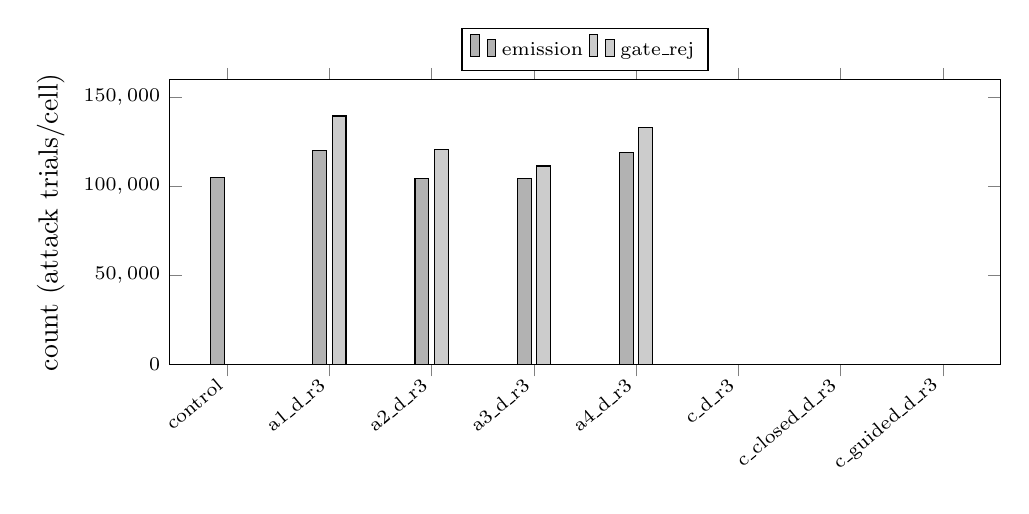
\begin{tikzpicture}
\begin{axis}[
  ybar,
  width=\linewidth,
  height=5.2cm,
  bar width=5pt,
  ymin=0,
  ymax=160000,
  ylabel={count (attack trials/cell)},
  symbolic x coords={control,a1\_d\_r3,a2\_d\_r3,a3\_d\_r3,a4\_d\_r3,c\_d\_r3,c\_closed\_d\_r3,c\_guided\_d\_r3},
  xtick=data,
  x tick label style={rotate=40,anchor=east,font=\scriptsize},
  scaled y ticks=false,
  yticklabel style={font=\scriptsize,/pgf/number format/fixed,/pgf/number format/1000 sep={,}},
  legend style={font=\scriptsize,at={(0.5,1.03)},anchor=south,legend columns=2},
  enlarge x limits=0.08,
]
\addplot+[fill=gray!60,draw=black] coordinates {
  (control,105173) (a1\_d\_r3,120140) (a2\_d\_r3,104697) (a3\_d\_r3,104615) (a4\_d\_r3,119091) (c\_d\_r3,0) (c\_closed\_d\_r3,0) (c\_guided\_d\_r3,0)
};
\addplot+[fill=black!20,draw=black] coordinates {
  (control,0) (a1\_d\_r3,139612) (a2\_d\_r3,120632) (a3\_d\_r3,111528) (a4\_d\_r3,133221) (c\_d\_r3,0) (c\_closed\_d\_r3,0) (c\_guided\_d\_r3,0)
};
\legend{emission, gate\_rej}
\end{axis}
\end{tikzpicture}
\caption{Emission and gate rejections per cell on the weak workhorse (\texttt{blast\_1p7b\_5m.db}, \(282{,}000\) attack trials/cell). Behavioral generators behind the gate emit \(>10^5\) out-of-scope calls each, which the gate must catch (\texttt{control} is ungated, so it has no gate-rejection bar). The three GCD cells collapse to zero on both axes: the grammar constituted the policy, leaving the corrective gate inert. This figure covers the emission and gate-rejection axes only; the output-token cost and valid-output rates appear in Table~\ref{tab:factorial}.}
\label{fig:factorial-cost}
\end{figure}

The slogan ``same policy, enforcement-completeness differs'' is thereby made operational: behavioral controls add cost \emph{in front of} the gate without eliminating emission; the gate restores the positive policy but pays a produce-then-catch tax (emission, tokens, retry attempts, and availability stranding at \(R=0\)); and \texttt{C} eliminates that tax by construction, making the corrective layer inert.

\begin{remark}[Reliability is two-sided]
\label{rem:two-sided}
Neither placement is unilaterally superior on reliability. Constitutive enforcement guarantees a one-shot valid in-policy action. However, a blind union grammar can silently \emph{deflect} a masked malicious intent into a valid but unrequested in-scope action: a reliability cost that is reported \emph{against} \texttt{C} (the deflection DV, Section~\ref{sec:method}) and that the per-request least-privilege grammar (\texttt{c\_guided}) drives to \(0\) by construction. Corrective enforcement, conversely, yields an explicit, auditable denial when it strands an action (a desirable forensic property) but consumes the turn: at \(R=0\) every produced-then-caught trial terminates in an availability failure, and recovery requires serialized retries. We measure both; we claim neither as dominant.
\end{remark}
